\FloatBarrier

\begin{figure}[h!]
	\centering
	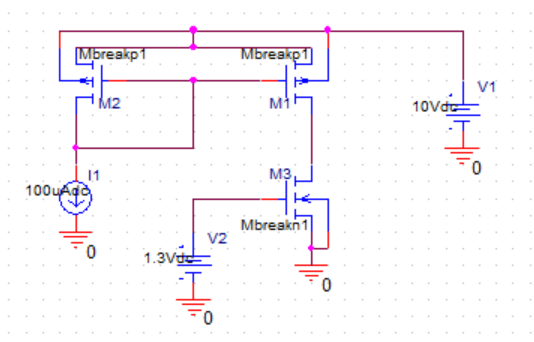
\includegraphics[scale=0.75]{../images/circuit2.PNG}
	\caption{Common-Source Amplifier with PMOS Current Mirror}
	\label{fig:circuit2}
\end{figure}

\FloatBarrier

The input voltage $V_2$ is swept from $0$\si{\volt} to $10$\si{\volt} to determine the voltage transfer characteristic.

\FloatBarrier

\begin{figure}[h!]
	\centering
	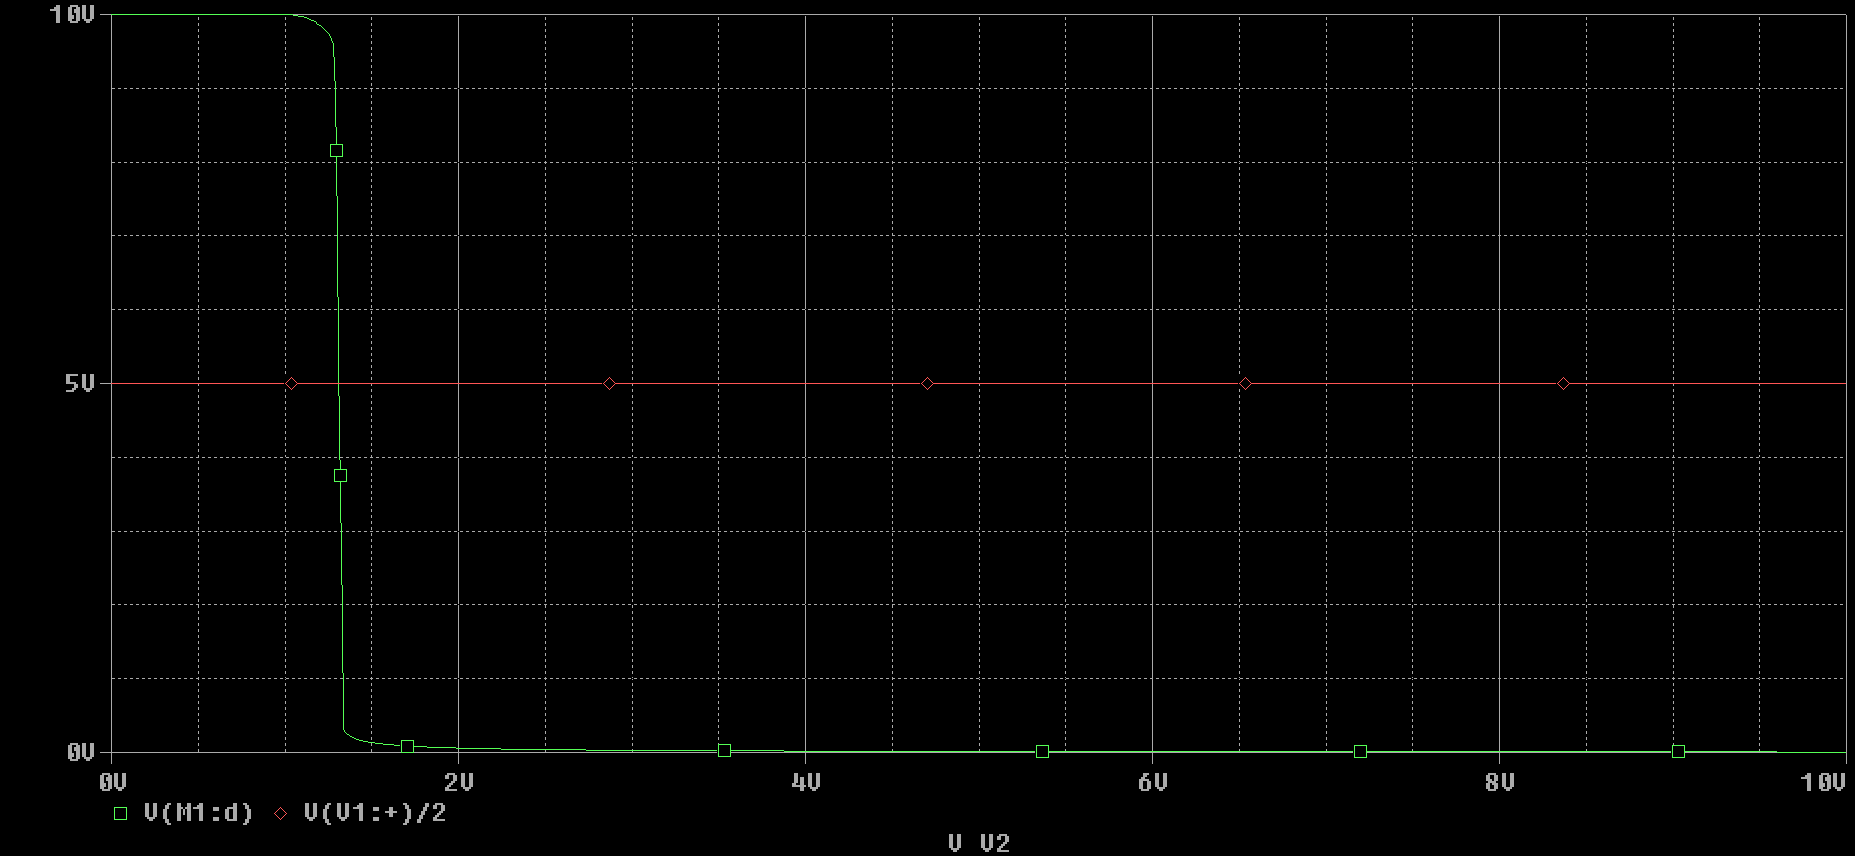
\includegraphics[scale=0.75]{../images/circuit2_dc_sweep.PNG}
	\caption{Voltage Transfer Characteristic of Figure (\ref{fig:circuit2}) Circuit}
	\label{fig:circuit2_dc_sweep}
\end{figure}

\FloatBarrier

The amplifier is biased at about $1.3116$\si{\volt}. A bias simulation is run, and its results are used to calculate the small signal parameters in table ().

\FloatBarrier

\begin{figure}[h!]
	\centering
	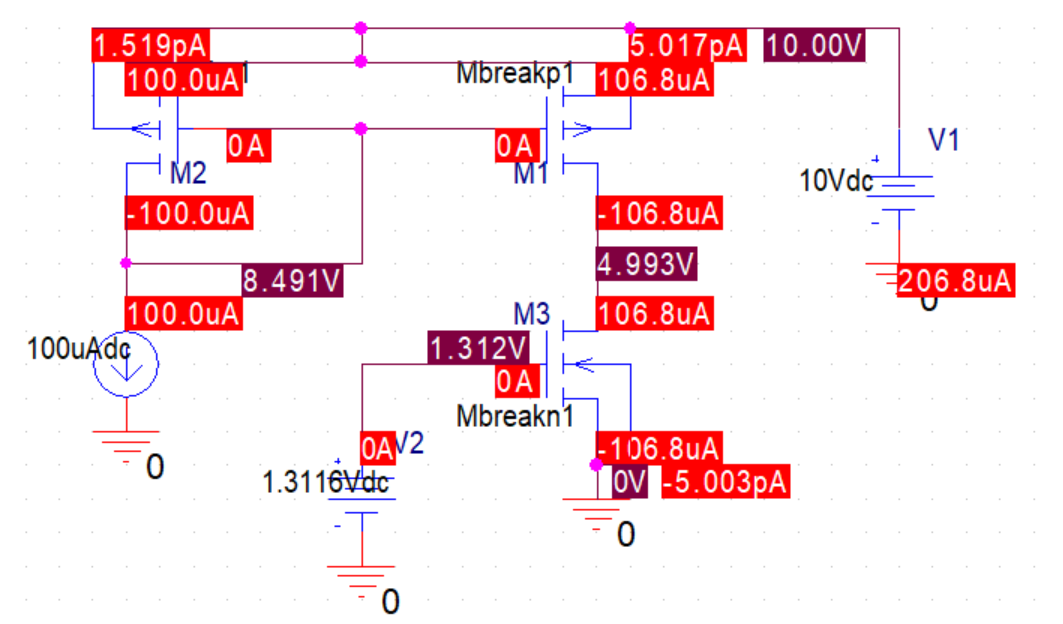
\includegraphics[scale=0.75]{../images/circuit2_bias_sim.PNG}
	\caption{Figure (\ref{fig:circuit2}) Circuit Bias Simulation}
	\label{fig:circuit2_bias_sim}
\end{figure}

\FloatBarrier

\FloatBarrier

\begin{table}[h!]
	\centering
	\caption{Small-Signal Parameters of Figure (\ref{fig:circuit2}) Circuit}
	\label{tab:ss_params}
	\csvautotabular{../tables/ss_params.csv}
\end{table}

\FloatBarrier

After analyzing the small-signal model of the circuit in figure (\ref{fig:circuit2}) using Kirchhoff's Current Law, the following equations are used to acquire the small-signal gain:

\begin{equation}
	\label{eq:ss_model_node_1}
	-0.624V_{in} - \frac{V_{out}}{514} + 0.38175V_{sg} + \frac{0 - V_{out}}{515} = 0
\end{equation}

\begin{equation}
	\label{eq:ss_model_node_2}
	\frac{V_{sg}}{515} + 0.38175V_{sg} = 0
\end{equation}

After solving equations (\ref{eq:ss_model_node_1}) and (\ref{eq:ss_model_node_2}), the gain is determined to be:

\begin{equation}
	\label{eq:gain}
	A = \frac{V_{out}}{V_{in}} \approx -160 [\frac{V}{V}]
\end{equation}

The low-frequency, small-signal gain can be determined through simulation as well. A $1$\si{\volt} amplitude signal is applied. Therefore, its output voltage's numerical value at low frequencies times $-1$ is the gain since $|A| = |\frac{V_{out}}{V_{in}}| = |\frac{V_{out}}{1}| = |V_{out}|$.

\FloatBarrier

\begin{figure}[h!]
	\centering
	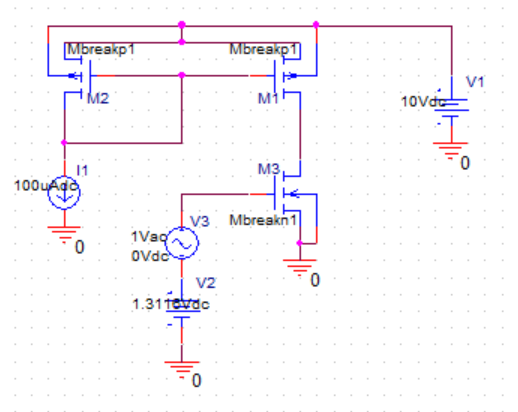
\includegraphics[scale=0.75]{../images/circuit3.PNG}
	\caption{AC Signal Version of Circuit in Figure (\ref{fig:circuit2})}
	\label{fig:circuit3}
\end{figure}

\FloatBarrier

\FloatBarrier

\begin{figure}[h!]
	\centering
	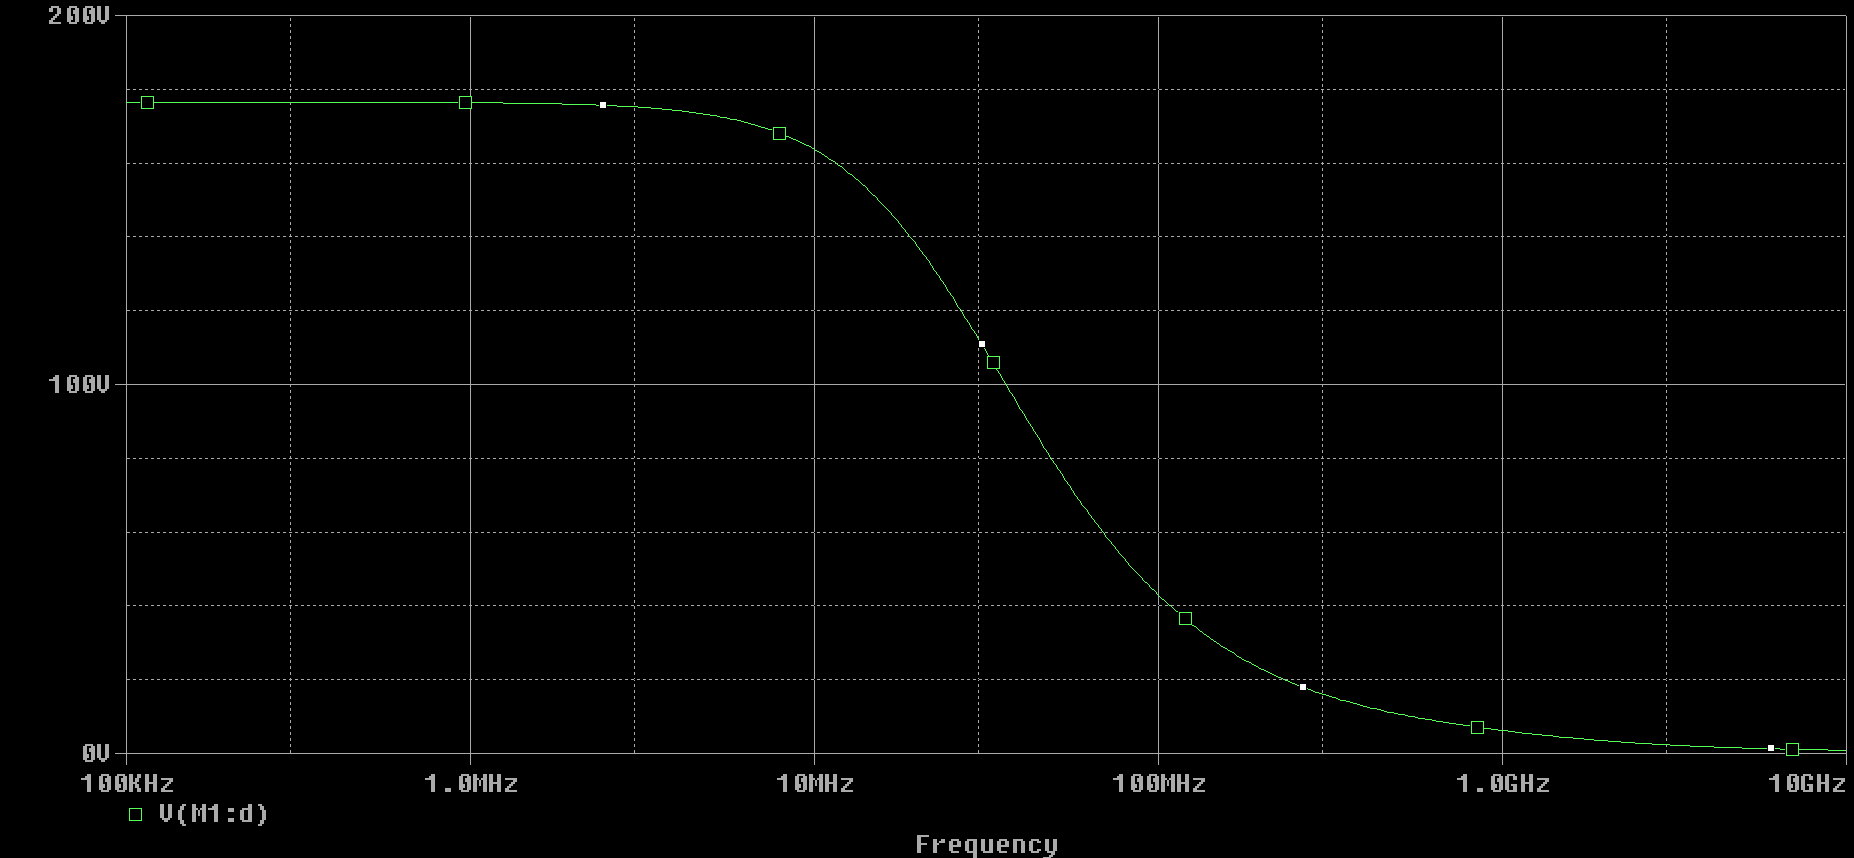
\includegraphics[scale=0.75]{../images/circuit3_ac_sweep.PNG}
	\caption{AC Sweep of Circuit in Figure (\fig{fig:circuit3})}
	\label{fig:circuit3_ac_sweep}
\end{figure}

\FloatBarrier

From figure (\ref{fig:circuit3_ac_sweep}), the gain is estimated to be about $-177[\frac{V}{V}]$. This gain is a bit larger in magnitude than what is expected from the small-signal model of the amplifier. After turning off each SPICE model parameter one-by-one, none seems to be directly responsible for this increased gain. Some inner-working of the transistor model is likely different from the small-signal model used for the calculations, though the two are reasonably close together.
